%package list
\documentclass{article}
\usepackage[english,spanish]{babel}
\usepackage[utf8]{inputenc}
\usepackage[top=3cm, bottom=3cm, outer=3cm, inner=3cm]{geometry}
\usepackage{multicol}
\usepackage{graphicx}
\usepackage{url}
%\usepackage{cite}
\usepackage{hyperref}
\usepackage{array}
%\usepackage{multicol}
\newcolumntype{x}[1]{>{\centering\arraybackslash\hspace{0pt}}p{#1}}
\usepackage{natbib}
\usepackage{pdfpages}
\usepackage{multirow}
\usepackage[normalem]{ulem}
\useunder{\uline}{\ul}{}
\usepackage{svg}
\usepackage{xcolor}
\usepackage{listings}
\lstdefinestyle{ascii-tree}{
    literate={├}{|}1 {─}{--}1 {└}{+}1 
  }
\lstset{basicstyle=\ttfamily,
  showstringspaces=false,
  commentstyle=\color{red},
  keywordstyle=\color{blue}
}
%\usepackage{booktabs}
\usepackage{caption}
\usepackage{subcaption}
\usepackage{float}
\usepackage{array}

\newcolumntype{M}[1]{>{\centering\arraybackslash}m{#1}}
\newcolumntype{N}{@{}m{0pt}@{}}


%%%%%%%%%%%%%%%%%%%%%%%%%%%%%%%%%%%%%%%%%%%%%%%%%%%%%%%%%%%%%%%%%%%%%%%%%%%%
%%%%%%%%%%%%%%%%%%%%%%%%%%%%%%%%%%%%%%%%%%%%%%%%%%%%%%%%%%%%%%%%%%%%%%%%%%%%
\newcommand{\itemEmail}{vmamanian@unsa.edu.pe}
\newcommand{\itemStudent}{Victor Mamani Anahua}
\newcommand{\itemCourse}{Programación Web 2}
\newcommand{\itemCourseCode}{20230489}
\newcommand{\itemSemester}{III}
\newcommand{\itemUniversity}{Universidad Nacional de San Agustín de Arequipa}
\newcommand{\itemFaculty}{Facultad de Ingeniería de Producción y Servicios}
\newcommand{\itemDepartment}{Departamento Académico de Ingeniería de Sistemas e Informática}
\newcommand{\itemSchool}{Escuela Profesional de Ingeniería de Sistemas}
\newcommand{\itemAcademic}{2024 - A}
\newcommand{\itemInput}{Del 8 Junio 2024}
\newcommand{\itemOutput}{Al 15 Junio 2024}
\newcommand{\itemPracticeNumber}{08}
\newcommand{\itemTheme}{Django - Relaciones}
%%%%%%%%%%%%%%%%%%%%%%%%%%%%%%%%%%%%%%%%%%%%%%%%%%%%%%%%%%%%%%%%%%%%%%%%%%%%
%%%%%%%%%%%%%%%%%%%%%%%%%%%%%%%%%%%%%%%%%%%%%%%%%%%%%%%%%%%%%%%%%%%%%%%%%%%%

\usepackage[english,spanish]{babel}
\usepackage[utf8]{inputenc}
\AtBeginDocument{\selectlanguage{spanish}}
\renewcommand{\figurename}{Figura}
\renewcommand{\refname}{Referencias}
\renewcommand{\tablename}{Tabla} %esto no funciona cuando se usa babel
\AtBeginDocument{%
	\renewcommand\tablename{Tabla}
}

\usepackage{fancyhdr}
\pagestyle{fancy}
\fancyhf{}
\setlength{\headheight}{30pt}
\renewcommand{\headrulewidth}{1pt}
\renewcommand{\footrulewidth}{1pt}
\fancyhead[L]{\raisebox{-0.2\height}{
\includegraphics[width=3cm]{img/logo_episunsa.png}}}
\fancyhead[C]{\fontsize{7}{7}\selectfont	\itemUniversity \\ \itemFaculty \\ \itemDepartment \\ \itemSchool \\ \textbf{\itemCourse}}
\fancyhead[R]{\raisebox{-0.2\height}{
\includegraphics[width=1.2cm]{img/logo_abet}}}
\fancyfoot[L]{Estudiante Victor Mamani A.}
\fancyfoot[C]{\itemCourse}
\fancyfoot[R]{Página \thepage}

% para el codigo fuente
\usepackage{listings}
\usepackage{color, colortbl}
\definecolor{dkgreen}{rgb}{0,0.6,0}
\definecolor{gray}{rgb}{0.5,0.5,0.5}
\definecolor{mauve}{rgb}{0.58,0,0.82}
\definecolor{codebackground}{rgb}{0.95, 0.95, 0.92}
\definecolor{tablebackground}{rgb}{0.8, 0, 0}

\lstset{frame=tb,
	language=bash,
	aboveskip=3mm,
	belowskip=3mm,
	showstringspaces=false,
	columns=flexible,
	basicstyle={\small\ttfamily},
	numbers=none,
	numberstyle=\tiny\color{gray},
	keywordstyle=\color{blue},
	commentstyle=\color{dkgreen},
	stringstyle=\color{mauve},
	breaklines=true,
	breakatwhitespace=true,
	tabsize=3,
	backgroundcolor= \color{codebackground},
}

\begin{document}
	
	\vspace*{10px}
	
	\begin{center}	
		\fontsize{17}{17} \textbf{ Informe de Laboratorio \itemPracticeNumber}
	\end{center}
	\centerline{\textbf{\Large Tema: \itemTheme}}
	%\vspace*{0.5cm}	

	\begin{flushright}
		\begin{tabular}{|M{2.5cm}|N|}
			\hline 
			\rowcolor{tablebackground}
			\color{white} \textbf{Nota}  \\
			\hline 
			     \\[30pt]
			\hline 			
		\end{tabular}
	\end{flushright}	

	\begin{table}[H]
		\begin{tabular}{|x{4.7cm}|x{4.8cm}|x{4.8cm}|}
			\hline 
			\rowcolor{tablebackground}
			\color{white} \textbf{Estudiante} & \color{white}\textbf{Escuela}  & \color{white}\textbf{Asignatura}   \\
			\hline 
			{\itemStudent \par \itemEmail} & \itemSchool & {\itemCourse \par Semestre: \itemSemester \par Código: \itemCourseCode}     \\
			\hline 			
		\end{tabular}
	\end{table}		
	
	\begin{table}[H]
		\begin{tabular}{|x{4.7cm}|x{4.8cm}|x{4.8cm}|}
			\hline 
			\rowcolor{tablebackground}
			\color{white}\textbf{Laboratorio} & \color{white}\textbf{Tema}  & \color{white}\textbf{Duración}   \\
			\hline 
			\itemPracticeNumber & \itemTheme & 04 horas   \\
			\hline 
		\end{tabular}
	\end{table}
	
	\begin{table}[H]
		\begin{tabular}{|x{4.7cm}|x{4.8cm}|x{4.8cm}|}
			\hline 
			\rowcolor{tablebackground}
			\color{white}\textbf{Semestre académico} & \color{white}\textbf{Fecha de inicio}  & \color{white}\textbf{Fecha de entrega}   \\
			\hline 
			\itemAcademic & \itemInput &  \itemOutput  \\
			\hline 
		\end{tabular}
	\end{table}
	
	\section{Tarea}
	\begin{itemize}		
		\item Informe de laboratorio
        \item Video en Flip
        \item Ejercicios Propuestos
	\end{itemize}
		
	\section{Equipos, materiales y temas utilizados}
	\begin{itemize}
		\item Sistema Operativo Ubuntu GNU Linux 23 lunar 64 bits Kernell 6.2.v
		\item Sistema Operativo Windows 11.
		\item Visual Studio Code
		\item OpenJDK 64-Bits 19.0.7.
		\item Git 2.39.2.
		\item Cuenta en GitHub con el correo institucional.	
	\end{itemize}
	
	\section{URL'S}
	\begin{itemize}
        \item No pude enviar el video por Flip
        \begin{figure}[H]
            \centering
            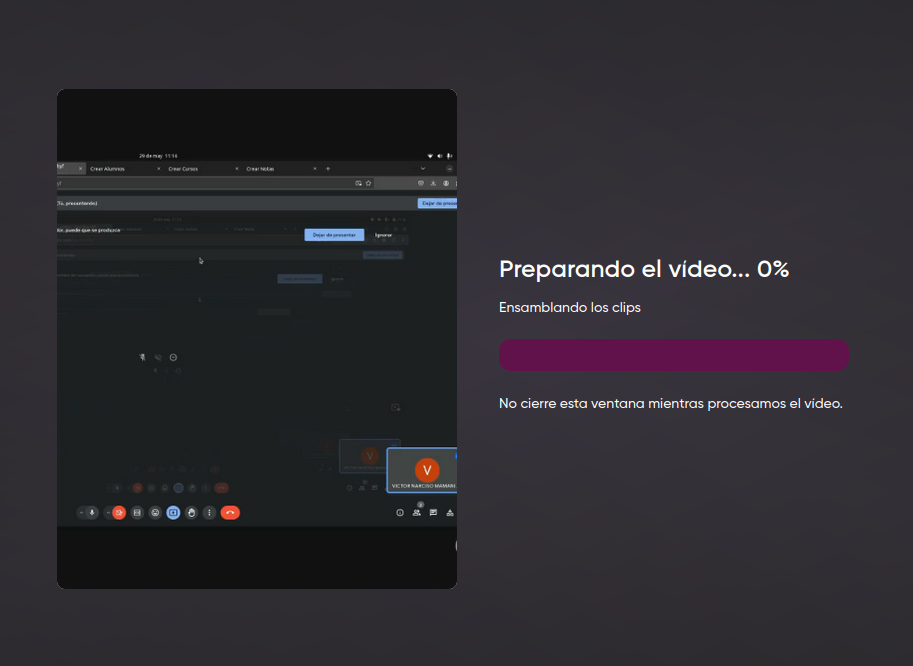
\includegraphics[width=0.7\textwidth]{img/Flip.png}
            \caption{Codigo y Ejecucion}
        \end{figure}
        \item URL para el video Drive.
        \item \url{https://drive.google.com/file/d/1bJ8cHqwOaGw1mopwqTKrRYf4IGWXiLt9/view?usp=sharing}
		\item URL para el Repositorio GitHub.
		\item \url{https://github.com/VictorMA18/Lab08-Django-Relaciones}
	\end{itemize}
	
	\section{Actividades del Laboratorio 08}
	\subsection{Hacer migraciones}
	\begin{itemize}	
        \item Primero activamos nuestro entorno virtual en el cual clonamos el repositorio
		\item Despues hacemos las migraciones respectivas
	\end{itemize}	
    \begin{lstlisting}[language=bash,caption={migraciones}][H]
        python3 manage.py makemigrations
        python3 manage.py migrations
	\end{lstlisting}

    \subsection{Relaciones uno a muchos y de muchos a muchos}
    \begin{itemize}	
    \item \textbf{Language}: Modelo que representa un lenguaje de programación.
        \begin{itemize}
            \item \textbf{name}: Nombre del lenguaje (campo \texttt{CharField} con longitud máxima de 10 caracteres).
        \end{itemize}
        
    \item \textbf{Framework}: Modelo que representa un framework asociado a un lenguaje.
        \begin{itemize}
            \item \textbf{name}: Nombre del framework (campo \texttt{CharField} con longitud máxima de 10 caracteres).
            \item \textbf{language}: Clave foránea que relaciona el framework con un lenguaje (relación \texttt{ForeignKey} hacia el modelo \textbf{Language}, con eliminación en cascada).
        \end{itemize}
        
    \item \textbf{Movie}: Modelo que representa una película.
        \begin{itemize}
            \item \textbf{name}: Nombre de la película (campo \texttt{CharField} con longitud máxima de 10 caracteres).
        \end{itemize}
        
    \item \textbf{Character}: Modelo que representa un personaje de película.
        \begin{itemize}
            \item \textbf{name}: Nombre del personaje (campo \texttt{CharField} con longitud máxima de 10 caracteres).
            \item \textbf{movies}: Relación de muchos a muchos con películas, indicando en qué películas aparece el personaje (relación \texttt{ManyToManyField} hacia el modelo \textbf{Movie}).
        \end{itemize}
	\end{itemize}
    \lstinputlisting[language=Python, caption={Código de views.py},numbers=left,]{../example/models.py}
    \begin{itemize}
        \item \textbf{Ahora veremos la base de datos}: Base de datos
        \begin{figure}[H]
            \centering
            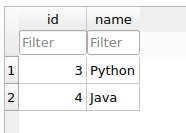
\includegraphics[width=0.7\textwidth]{img/Cap1.png}
            \caption{Base de Datos}
        \end{figure}
        \begin{figure}[H]
            \centering
            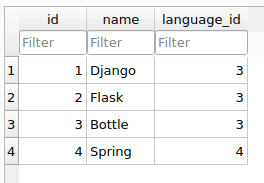
\includegraphics[width=0.7\textwidth]{img/Cap2.png}
            \caption{Base de Datos}
        \end{figure}
        \begin{figure}[H]
            \centering
            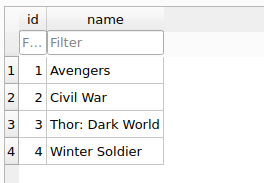
\includegraphics[width=0.7\textwidth]{img/Cap3.png}
            \caption{Base de Datos}
        \end{figure}
        \begin{figure}[H]
            \centering
            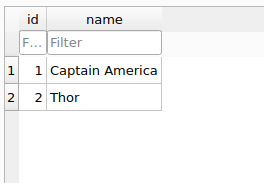
\includegraphics[width=0.7\textwidth]{img/Cap4.png}
            \caption{Base de Datos}
        \end{figure}
        \begin{figure}[H]
            \centering
            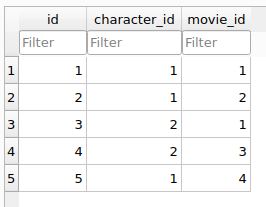
\includegraphics[width=0.7\textwidth]{img/Cap5.png}
            \caption{Base de Datos}
        \end{figure}
    \end{itemize}

    \subsection{Impresión de pdfs y envio de emails}
    \begin{itemize}	
        \item Primero descargamos la libreria de python xhtml12pdf que nos ayuda a renderizar nuestro html a pdf
    \end{itemize}	
    \begin{lstlisting}[language=bash,caption={migraciones}][H]
        pip install xhtml12pdf
	\end{lstlisting}
    \begin{itemize}
        \item Archivo \textbf{utils.py}:
        \item Función \textbf{render\_to\_pdf}:
            \begin{itemize}
                \item Descripción: Renderiza un template HTML con un contexto y genera un archivo PDF utilizando xhtml2pdf.
                \item Parámetros:
                    \begin{itemize}
                        \item \textbf{template\_src}: Ruta al template HTML que se va a renderizar.
                        \item \textbf{context\_dict}: Diccionario con el contexto que se va a pasar al template (opcional, por defecto es un diccionario vacío).
                    \end{itemize}
                \item Acciones:
                    \begin{itemize}
                        \item Carga el template especificado utilizando \texttt{get\_template}.
                        \item Renderiza el template con el contexto utilizando \texttt{template.render}.
                        \item Convierte el HTML renderizado a un documento PDF utilizando \texttt{pisa.pisaDocument}.
                        \item Retorna un objeto \texttt{HttpResponse} con el contenido del PDF si la conversión fue exitosa.
                        \item Si hay errores durante la conversión a PDF, retorna una respuesta de error con código 400 y un mensaje de "Invalid PDF".
                    \end{itemize}
            \end{itemize}
    \end{itemize}

    \lstinputlisting[language=Python, caption={Código de views.py},numbers=left,]{../example/utils.py}

    \begin{itemize}
        \item Archivo \textbf{views.py}:
        \item \textbf{Función \texttt{get\_pdf}}:
            \begin{itemize}
                \item Descripción: Genera un documento PDF de una factura utilizando un template HTML y lo devuelve como respuesta HTTP.
                \item Acciones:
                    \begin{itemize}
                        \item Carga el template 'invoice.html' usando \texttt{get\_template}.
                        \item Define un contexto con datos de la factura como número de factura, nombre del cliente, monto y fecha.
                        \item Renderiza el template a HTML utilizando \texttt{template.render}.
                        \item Genera un PDF llamando a \texttt{render\_to\_pdf}.
                        \item Si se genera correctamente el PDF:
                            \begin{itemize}
                                \item Crea una respuesta HTTP con el PDF y establece el tipo de contenido como 'application/pdf'.
                                \item Configura el nombre del archivo y si debe descargarse o mostrarse en línea según el parámetro \texttt{download} en la solicitud.
                                \item Retorna la respuesta HTTP con el PDF.
                            \end{itemize}
                        \item Si no se puede generar el PDF, retorna una respuesta HTTP indicando "Not found".
                    \end{itemize}
            \end{itemize}
            
        \item \textbf{Función \texttt{get\_pdf\_advanced}}:
            \begin{itemize}
                \item Descripción: Genera un documento PDF más avanzado de una factura con datos formateados y lo devuelve como respuesta HTTP.
                \item Acciones:
                    \begin{itemize}
                        \item Configura el entorno local para formateo de moneda usando \texttt{locale.setlocale}.
                        \item Define datos de la factura como nombre del cliente, número de factura, monto formateado como moneda, fecha y título del PDF.
                        \item Llama a \texttt{utils.render\_to\_pdf} para generar el PDF utilizando el template 'invoice.html' y el contexto definido.
                        \item Maneja la respuesta del PDF:
                            \begin{itemize}
                                \item Si la generación tiene éxito, configura la respuesta con el nombre del archivo y el tipo de contenido.
                                \item Decide si el archivo debe descargarse o mostrarse en línea según el parámetro \texttt{download} en la solicitud.
                                \item Retorna la respuesta HTTP con el PDF generado.
                                \item Si no se encuentra la factura (código 404), lanza una excepción HTTP404.
                            \end{itemize}
                    \end{itemize}
            \end{itemize}
            
        \item \textbf{Función \texttt{emails}}:
            \begin{itemize}
                \item Descripción: Maneja el envío de correos electrónicos desde un formulario POST y muestra un mensaje de confirmación.
                \item Acciones:
                    \begin{itemize}
                        \item Si la solicitud es POST, obtiene el asunto, mensaje y destinatario del formulario.
                        \item Utiliza \texttt{send\_mail} para enviar el correo electrónico utilizando los datos obtenidos.
                        \item Retorna una respuesta HTTP con un mensaje de confirmación y un enlace para volver al menú principal.
                        \item Si la solicitud no es POST, renderiza el template 'emails.html'.
                    \end{itemize}
            \end{itemize}
            
        \item \textbf{Función \texttt{index}}:
            \begin{itemize}
                \item Descripción: Renderiza la página principal ('index.html').
                \item Acciones:
                    \begin{itemize}
                        \item Retorna la respuesta renderizada del template 'index.html'.
                    \end{itemize}
            \end{itemize}
        \item \textbf{Correo del Remitente debe ser cambiado por el correo personal}
        \begin{lstlisting}[language=Python,caption={Codigo de settings.py del proyecto}][H]
            DEFAULT_AUTO_FIELD = 'django.db.models.BigAutoField'
            EMAIL_BACKEND = 'django.core.mail.backends.smtp.EmailBackend'
            EMAIL_HOST = 'smtp.gmail.com'  
            EMAIL_PORT = 587
            EMAIL_USE_TLS = True
            EMAIL_HOST_USER = 'correo@gmail.com'
            EMAIL_HOST_PASSWORD = ''
        \end{lstlisting}
    \end{itemize}
    
    \lstinputlisting[language=Python, caption={Código de views.py},numbers=left,]{../example/views.py}

    \begin{itemize}
        \item Archivos HTML \textbf{emails.html , index.html , invoice.html}:
        \item \textbf{Archivo \texttt{emails.html}}:
        \lstinputlisting[language=Python, caption={Código de views.py},numbers=left,]{../templates/emails.html}
        \item \textbf{Archivo \texttt{index.html}}:
        \lstinputlisting[language=Python, caption={Código de views.py},numbers=left,]{../templates/index.html}
        \item \textbf{Archivo \texttt{invoice.html}}:
        \lstinputlisting[language=Python, caption={Código de views.py},numbers=left,]{../templates/invoice.html}
        \item \textbf{Visualizacion}:
        \begin{figure}[H]
            \centering
            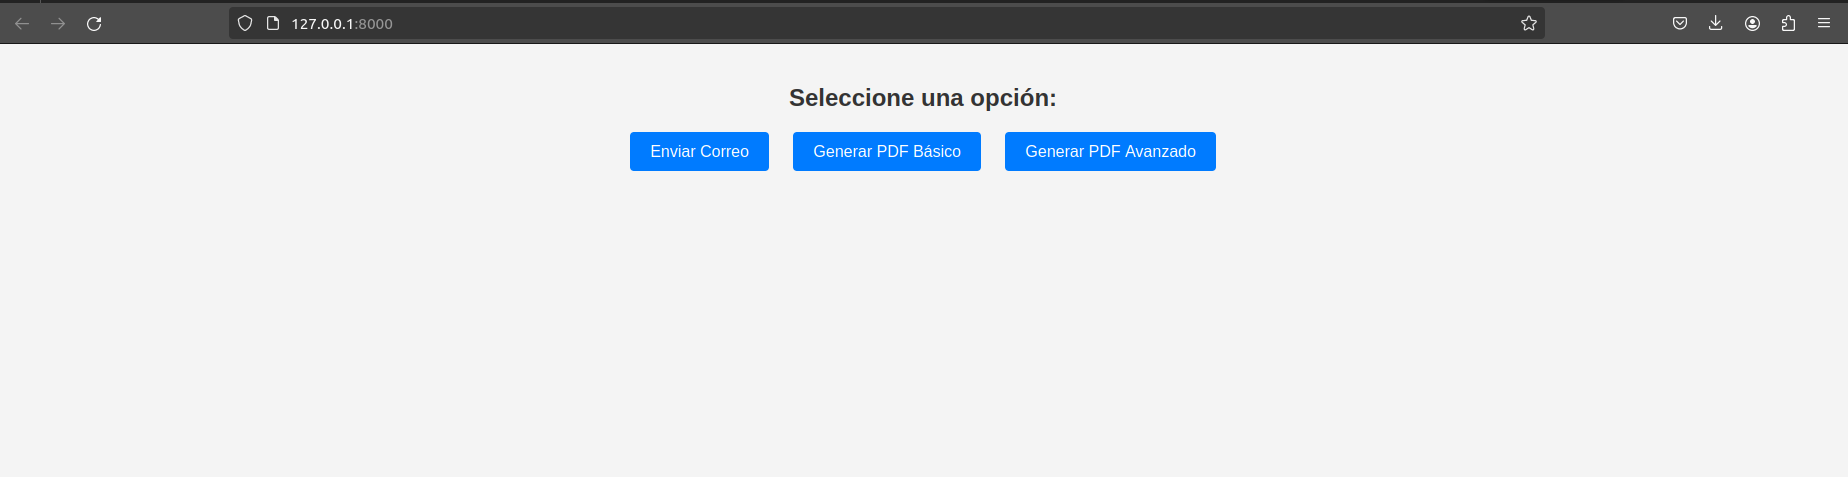
\includegraphics[width=1.0\textwidth]{img/Cap6.png}
            \caption{INDEX.HTML}
        \end{figure}
        \begin{figure}[H]
            \centering
            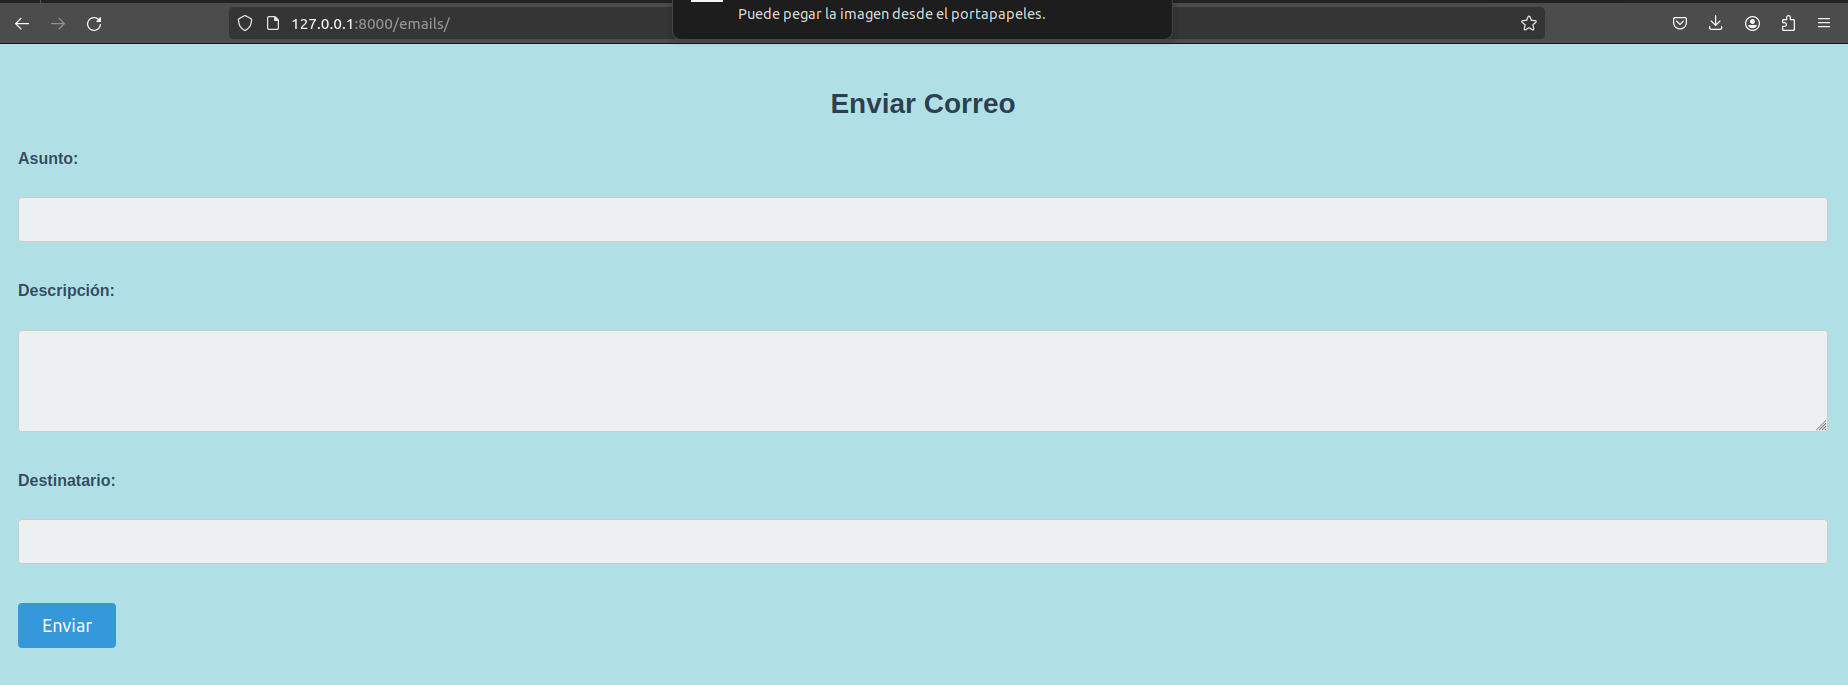
\includegraphics[width=1.0\textwidth]{img/Cap7.png}
            \caption{EMAILS.HTML}
        \end{figure}
        \begin{figure}[H]
            \centering
            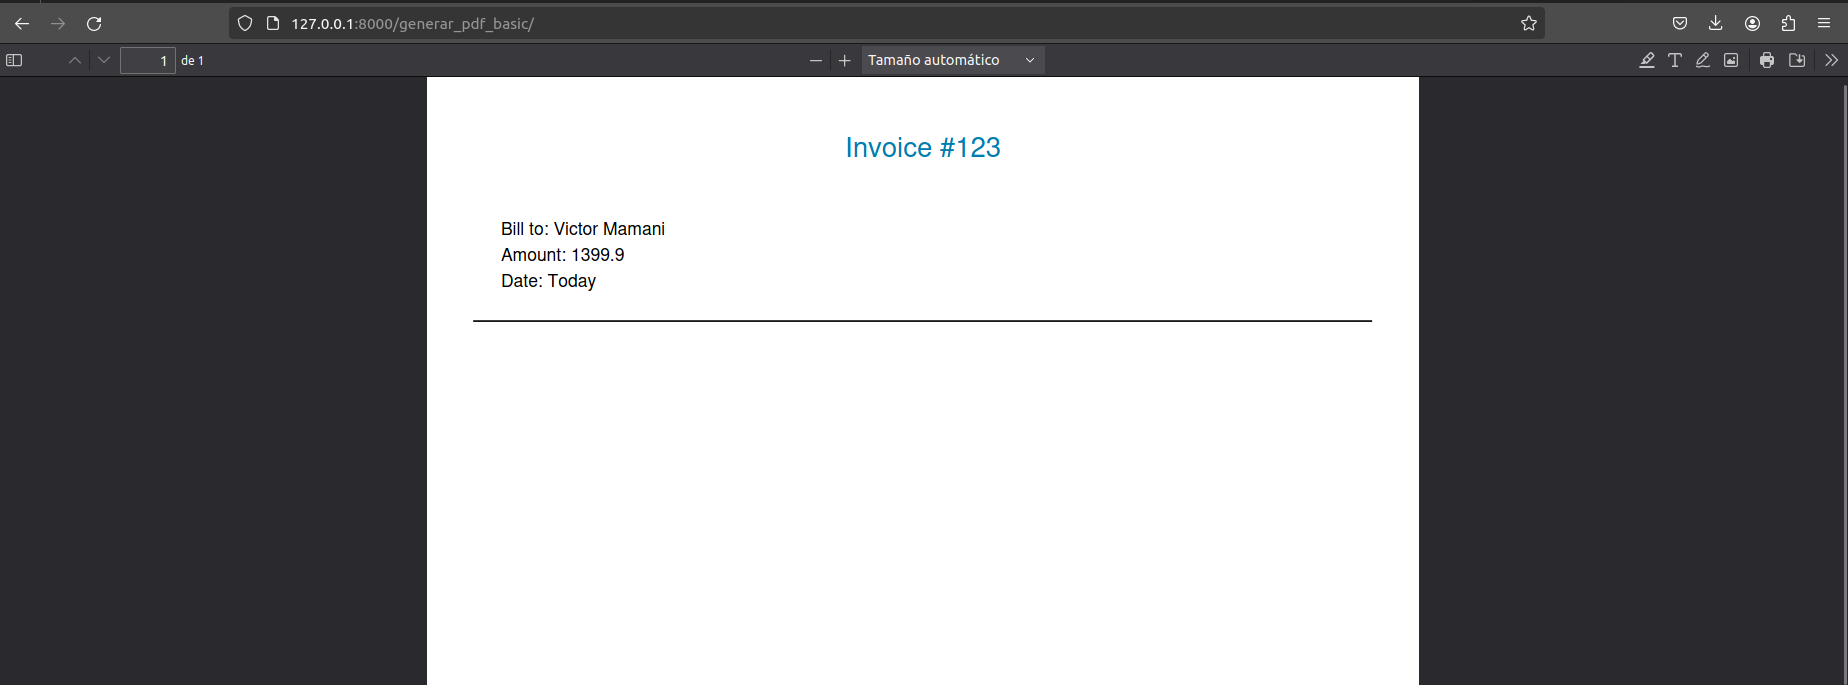
\includegraphics[width=1.0\textwidth]{img/Cap8.png}
            \caption{INVOICE.HTML}
        \end{figure}
        \begin{figure}[H]
            \centering
            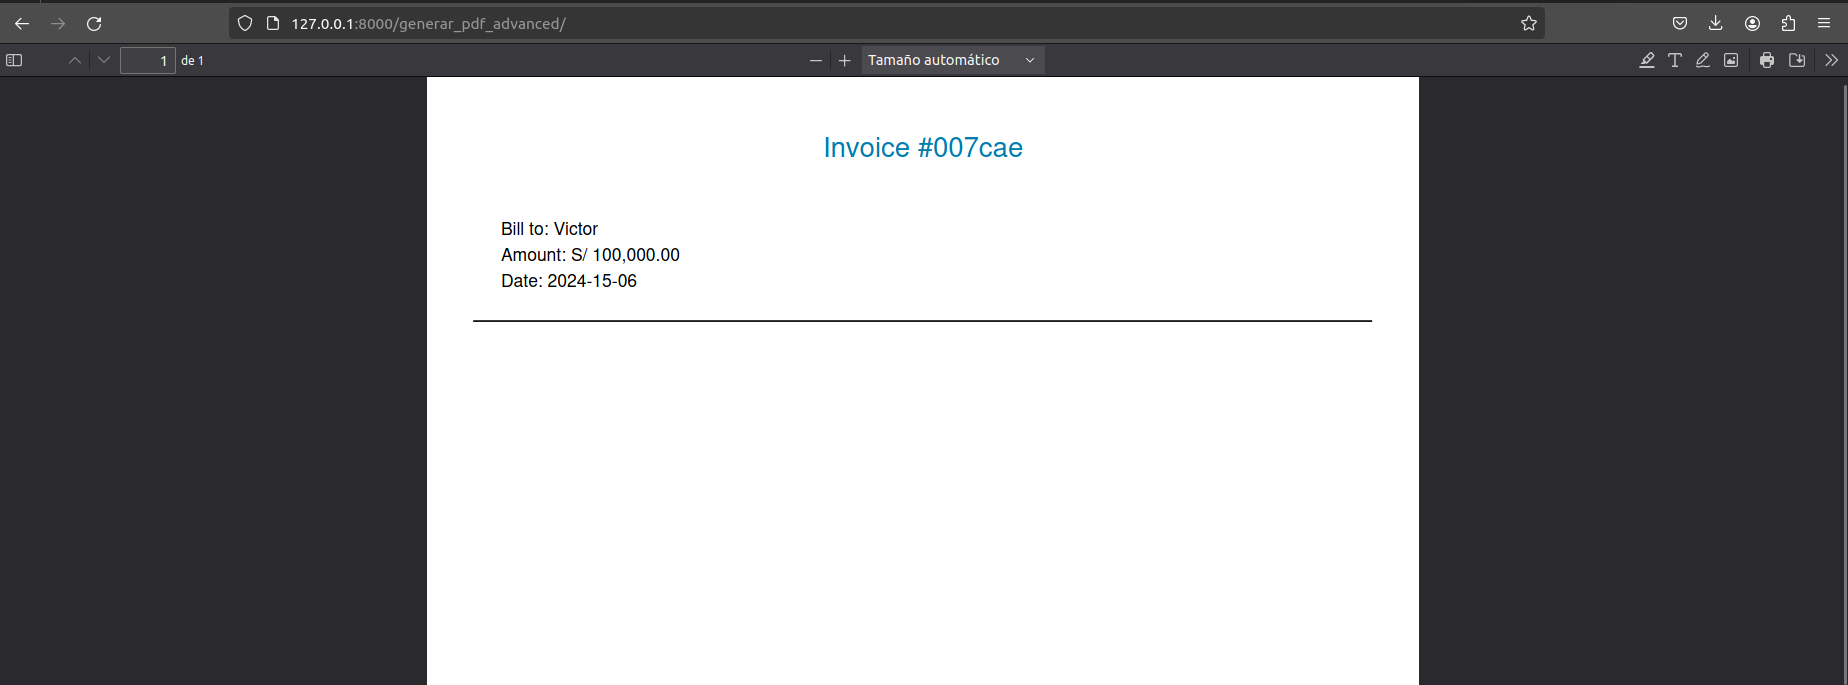
\includegraphics[width=1.0\textwidth]{img/Cap9.png}
            \caption{INVOICE.HTML}
        \end{figure}
    \end{itemize}

    \subsection{Links de las paginas}
    \begin{itemize}			
        \item INDEX:
        \item \url{http://127.0.0.1:8000/}
        \item CORREOS:
        \item \url{http://127.0.0.1:8000/emails/}
        \item PDF BASICO:
        \item \url{http://127.0.0.1:8000/generar_pdf_basic/}
        \item PDF AVANZADO:
        \item \url{http://127.0.0.1:8000/generar_pdf_advanced/}
    \end{itemize}

\section{Referencias}
\begin{itemize}			
	\item \url{https://docs.djangoproject.com/es/3.2/}
	\item \url{https://docs.djangoproject.com/es/3.2/ref/models/fields/#field-types}
	\item \url{https://www.w3schools.com/django/}
\end{itemize}	
	
%\clearpage
%\bibliographystyle{apalike}
%\bibliographystyle{IEEEtranN}
%\bibliography{bibliography}
			
\end{document}